\documentclass[11pt]{article}
\usepackage[a4paper,margin=25mm]{geometry}
\usepackage[T1]{fontenc}
\usepackage{lmodern,amsmath,amssymb,amsthm,mathtools,graphicx}
\usepackage[hidelinks]{hyperref}
\setlength{\emergencystretch}{2em}
\newcommand{\C}{\mathbb C}
\newcommand{\R}{\mathbb R}
\newcommand{\Tr}{\operatorname{Tr}}
\newcommand{\norm}[1]{\lVert#1\rVert}
\newtheorem{theorem}{Theorem}
\title{Every original eigenclass meets the arithmetic action boundary}
\author{Split-Zero research programme}
\date{21 September 2026}
\begin{document}\maketitle

The original polynomial source has a rank-two Hermitian action boundary.
The complete root grid forces a stronger lower bound for this boundary
than the largest real part of one root. We prove the bound, evaluate its
effect on every original eigenclass, and carry the resulting residual
through the fixed conductor projection. The source, its full relation
ideal, and the physical coordinate remain unchanged.

The attained-source boundary is the earlier result NAB1--19
\cite{NAB}; SD1--3 \cite{SD} identifies its norm with the rank-one
quantity used in the heat calculation. The new root-sum estimate is
NE6. Its eigenclass consequences are NE8--11. The supplied eigenvector
continuation \cite[(38)--(41)]{Incoming} supplies the general phase
identity and the test over all projections; we prove them here with
their exact receiver in the original kernel. No sign of that fixed
kernel is inferred from a sign obtained by choosing a different projection.

\section{Original source and the complete boundary}
Fix $0<\delta<1/2$, $\gamma>2$, odd $k\ge9$, and a positive integer
$e$. The simple-packet kernel uses $e=1$ and $k\equiv1\pmod4$.
The boundary calculation also retains the original repeated-root
case $e=1+k(m_0-1)$ when it occurs. Set
\begin{equation}\tag{NE1}
\begin{gathered}
c=k/2,\qquad q=e(k+1)^2,\qquad
\lambda_{ab}=c+(2a-k)\delta+i(2b-k)\gamma,\\
\chi(S)=\prod_{a,b=0}^k(S-\lambda_{ab})^e,\qquad
E=\C[S]/(\chi),\qquad A[P]=[SP].
\end{gathered}
\end{equation}
Use the full original positive measure $d\mu(y)=w_h^{*k}(y)\,dy$
on $S=c+iy$, with its mass and all original units retained.
All the following finite results hold for any fixed positive source
measure on this same line whose polynomial Grams through degree $N+1$
are finite and positive definite. This includes the full arithmetic
source and the separately identified Gamma source. It does not identify
their metrics. Fix $N\ge q-1$ and let
\[
T_N:E\longrightarrow\mathcal P_N,
\qquad G_N=T_N^*H_NT_N
\]
be the attained minimum section and its Gram matrix. Here $H_N$ is the
Gram matrix of the literal powers $1,S,\ldots,S^N$ and the kernel of
the source map is the whole ideal $\chi\mathcal P_{N-q}$.
For $N=q-1$ this ideal is zero. If $W_N$ contains the coefficient
columns of $\chi,S\chi,\ldots,S^{N-q}\chi$, the section is exactly
\[
T_N=E_N-W_N(W_N^*H_NW_N)^{-1}W_N^*H_NE_N,
\]
where $E_N$ inserts polynomials of degree below $q$. The omitted-column
case means $T_N=E_N$. The formula is proved by reducing modulo $\chi$
and checking $W_N^*H_NT_N=0$; every other lift has the additional
nonnegative squared norm of its orthogonal ideal component.

Let $\ell_N=[S^N]T_N$, let $b_N$ be the coefficient vector of
$\chi S^{N+1-q}$, and set $\xi_N=T_N^*H_{N+1}b_N$, with a zero
top coordinate appended to $T_N$ in this product. Monic division gives
\[
S T_N-T_N A=b_N\ell_N+Z_N,
\qquad \operatorname{im}Z_N\subset\chi\mathcal P_{N-q}.
\]
The latter term is orthogonal to $T_N$. On the physical line,
$\overline S+S=k$, hence
\begin{equation}\tag{NE2}
D_N=A^*G_N+G_NA-kG_N=-\xi_N\ell_N-\ell_N^*\xi_N^*.
\end{equation}
This proves the complete boundary without dropping a lower relation.
Use $\dagger$ for the $G_N$ adjoint and put
\begin{equation}\tag{NE3}
B=A+A^\dagger-kI=G_N^{-1}D_N.
\end{equation}
It is selfadjoint in $G_N$, has rank at most two, and has trace zero:
$\Tr B=2\Re\Tr A-kq=0$ by the complete grid in NE1.
An eigenvector at $a=k$ has Rayleigh quotient $2k\delta$ for $B$;
one at $a=0$ has quotient $-2k\delta$. Such vectors exist also on each
repeated-root primary block. Thus $B$ has exactly the two nonzero
eigenvalues $+\kappa_N,-\kappa_N$, with $\kappa_N>0$. If $P_\partial$
is its orthogonal support projection, then
\begin{equation}\tag{NE4}
B^2=\kappa_N^2P_\partial.
\end{equation}
All diagonalizations used here concern selfadjoint operators in the
specified metric and are proved by maximizing the Rayleigh quotient
on a finite unit sphere and inducting on its invariant orthogonal
complement.

For the even original measure, write $y=(S-c)/i$ and $M=(A-cI)/i$.
The attained compression $C_N$ of multiplication by real $y$ is
selfadjoint. Subtracting the leading multiple of the real monic source
orthogonal polynomial $p_{N+1}$ before compression gives
$M=C_N+r_N\ell_N^{y}$, where $r_N=[p_{N+1}]$ and
$\ell_N^{y}=[y^N]T_N$. Reflection in $y$ makes these two factors have
opposite parity. In particular $\ell_N^{y}r_N=0$. Therefore
\begin{equation}\tag{NE5}
B=i(r_N\ell_N^{y}-(r_N\ell_N^{y})^\dagger),\qquad
\kappa_N=\norm{r_N\ell_N^{y}}_{G_N}=\epsilon_N.
\end{equation}
Indeed the two normalized factor vectors are orthogonal, and the
matrix of $B$ on their span has off-diagonal entries $i\epsilon_N$
and $-i\epsilon_N$. This also extends this finite equality to $N=2q$;
the earlier SD cutoff range does not restrict the finite proof above.
The real-zero fact for positive-source orthogonal polynomials, used
to ensure the remainder is nonzero, is the classical result recorded
by Koornwinder and coauthors \cite[\S18.2(vi)]{DLMF}. A direct proof is
to multiply its real sign-changing factors: if fewer than its degree
occur, this lower-degree polynomial has nonzero inner product with
the orthogonal polynomial, contradicting orthogonality.

\section{The whole root grid strengthens the boundary bound}
\begin{theorem}
At every original cutoff, including all four cutoffs
$q-1,q,2q-1,2q$,
\begin{equation}\tag{NE6}
\boxed{\displaystyle\kappa_N\ge\frac{e\delta(k+1)^3}{2}.}
\end{equation}
\end{theorem}
\begin{proof}
Let $E_+$ be the direct sum of the full primary spaces at roots with
$a>(k/2)$. It is invariant under $A$ and has dimension $q/2$.
Existence and the direct sum follow from the coprime-factor polynomial
identity: Bezout inverses give the Chinese-remainder isomorphism
$E\cong\bigoplus_{a,b}\C[z]/(z^e)$; multiplication is
$\lambda_{ab}+z$ on each summand. Choose a $G_N$-orthonormal basis
of $E_+$ and let $P_+$ be its orthogonal projection. Its compressed
action is the restriction of $A$, so
\[
\Tr(P_+B)=2\Re\Tr(A|_{E_+})-k\dim E_+
=e\sum_{a=(k+1)/2}^{k}\sum_{b=0}^k2(2a-k)\delta.
\]
This is a trace identity; the original eigenvectors have not been
assumed orthogonal. If $u_+,u_-$ are the two unit boundary eigenvectors,
then $\Tr(P_+B)=\kappa_N(\norm{P_+u_+}^2-
\norm{P_+u_-}^2)\le\kappa_N$.
The positive odd integers $2a-k$ sum to $((k+1)/2)^2$.
Evaluating the displayed double sum proves NE6.
\end{proof}


\begin{figure}[p]\centering
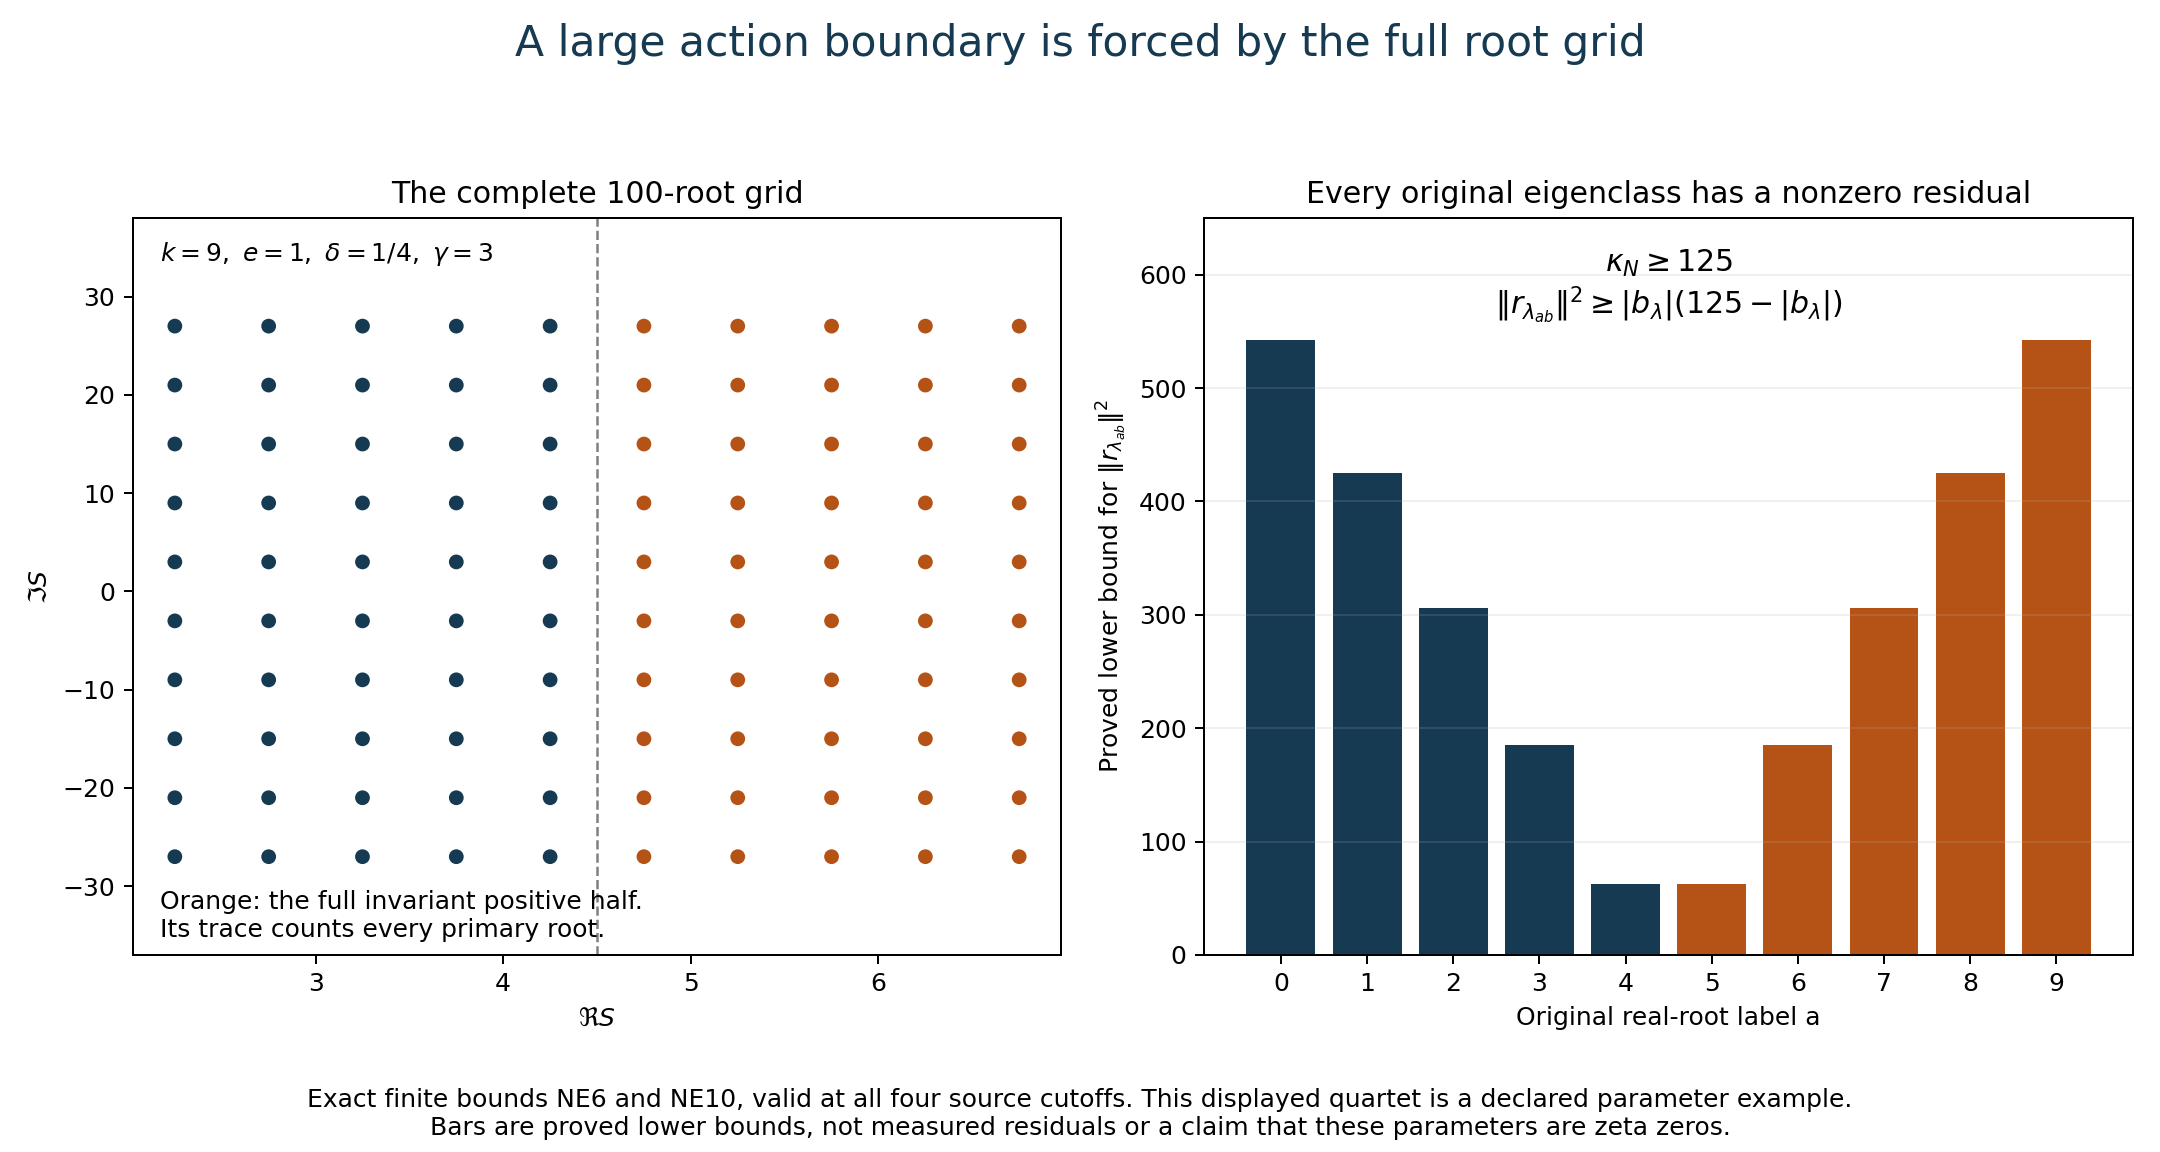
\includegraphics[width=\linewidth]{ORIGINAL_BOUNDARY_AND_RESIDUAL.png}
\caption{NE6 and NE10 evaluated at the displayed parameter example.
The grid uses the original $S=k/2+iy$ coordinate. All ten imaginary
labels occur at each real label. The projection used in NE6 is the
orthogonal projection onto the invariant positive half of the spectrum;
its trace is evaluated without assuming the root eigenvectors orthogonal.
The plot does not replace the original conductor projection NE12.
The scalar-source boundary is NAB1--19; its orthogonal-polynomial
convention is the classical one cited in NE5.}
\end{figure}

\section{An evaluated residual for every original eigenclass}
Let $v\ne0$ be any actual eigenvector at $\lambda_{ab}$, including
the eigenline inside a repeated-root primary space. Keep its physical
scale $E_v=\norm v_{G_N}^2$. For calculation only, put
\begin{equation}\tag{NE7}
x=v/\sqrt{E_v},\quad b_\lambda=2\Re\lambda-k=2(2a-k)\delta,
\quad r_\lambda=(A^\dagger-\overline\lambda I)x,
\quad \eta_\lambda=\norm{P_\partial x}_{G_N}^2.
\end{equation}
No metric, physical class, or source map is changed by this notation.
Since $Ax=\lambda x$, NE3 gives $r_\lambda=(B-b_\lambda I)x$.
Moreover $\langle x,Bx\rangle=b_\lambda$ and
$r_\lambda\perp x$. Consequently
\begin{equation}\tag{NE8}
\boxed{\norm{r_\lambda}^2=\kappa_N^2\eta_\lambda-b_\lambda^2,
\quad |b_\lambda|/\kappa_N\le\eta_\lambda\le1,}
\end{equation}
and hence
\begin{equation}\tag{NE9}
\boxed{|b_\lambda|(\kappa_N-|b_\lambda|)
\le\norm{r_\lambda}^2\le\kappa_N^2-b_\lambda^2.}
\end{equation}
For proof, use NE4 to evaluate $\norm{(B-b_\lambda)x}^2$.
In the boundary eigenbasis,
$|\langle x,Bx\rangle|\le\kappa_N\norm{P_\partial x}^2$,
which proves the remaining inequalities.

Since $k$ is odd, $|2a-k|\ge1$. NE6 is larger than $2k\delta$
for the stated domain. Inserting it into NE9 gives the finite
strictly positive bound for every eigenclass
\begin{equation}\tag{NE10}
\boxed{\norm{r_\lambda}^2\ge
\delta^2|2a-k|\bigl(e(k+1)^3-4|2a-k|\bigr)>0.}
\end{equation}
For a terminal class $a=k$ the right side is
$\delta^2k(e(k+1)^3-4k)$. This holds before invoking an asymptotic
estimate, numerical period, or EIQ statement.

The previously proved allowance estimate used by H1--7
\cite{Heat} is
$\log\epsilon_N^2=2q\psi(s_N)+O_h(k\log^2(q+2))$ on its stated
source and cutoff domain. NE5 and NE9 now give, on precisely that
domain and retaining that proof dependence,
\begin{equation}\tag{NE11}
q\psi(s_N)-O_h(k\log^2(q+2))
\le\log\norm{r_\lambda}^2
\le2q\psi(s_N)+O_h(k\log^2(q+2)).
\end{equation}
The lower bound uses $|b_\lambda|\ge2\delta$ and eventually
$\kappa_N\ge2|b_\lambda|$; the finite form is NE9 whenever that
eventual guard has not been certified. NE11 is an interval of rates,
not an evaluated leading coefficient inside that interval. The new
finite theorem NE10 is independent of the imported profile.

\section{The receiver in the fixed conductor kernel}
Return now to the simple-packet case and the actual kernel of MR1--10
\cite{MR}. Its frame is $I_K=V^{-1}\pi^T$ with
$\ker\pi=\operatorname{im}[M_A,S_kZ_k]$, and its dimension is
$m=8k-16$. The transpose in this frame is the complex-linear dual,
not an adjoint. Set
\begin{equation}\tag{NE12}
H_K=I_K^*G_NI_K,\qquad P=I_KH_K^{-1}I_K^*G_N,
\quad p=Px,\quad\theta=\norm p^2.
\end{equation}
Positive definiteness of $H_K$ proves that this is the actual
orthogonal projection; multiplication verifies $P^2=P$ and
$P^*G_N=G_NP$. It retains the complete invariant image and all
relations already minimized in $G_N$.
For the specified physical eigenclass define exactly
\[
z=\langle Pv,A(I-P)v\rangle_{G_N},\qquad
w=\langle(I-P)v,APv\rangle_{G_N}.
\]
Then the incoming identity has the following native receiver:
\begin{equation}\tag{NE13}
\boxed{\Re(\overline zw)=\left|\frac{z+w}{2}\right|^2
-\frac{E_v^2}{4}\left|\langle Bx,p\rangle-b_\lambda\theta\right|^2.}
\end{equation}
Indeed $w-z=E_v\langle r_\lambda,p\rangle$ follows by expanding
$Ax=\lambda x$ and the adjoint. The elementary identity
$\Re(\overline zw)=|(z+w)/2|^2-|w-z|^2/4$, followed by NE7,
proves NE13. In literal source coordinates the residual scalar is
\begin{equation}\tag{NE14}
\langle Bx,p\rangle-b_\lambda\theta
=-(x^*\xi_N)(\ell_Np)
-\overline{\ell_Nx}(\xi_N^*p)-b_\lambda\theta.
\end{equation}
This follows from $G_NB=D_N$ and NE2. It evaluates the needed
functional using the two actual boundary rows, while NE12 supplies
their actual kernel projection. In particular no full spectral
polynomial is substituted for these complex matrix elements.
As $r_\lambda\perp x$ and
$\norm{p-\theta x}^2=\theta(1-\theta)$, NE8 yields
\begin{equation}\tag{NE15}
[-\Re(\overline zw)]_+
\le\frac{E_v^2}{4}
(\kappa_N^2\eta_\lambda-b_\lambda^2)\theta(1-\theta).
\end{equation}
This is a rigorous error bound for the fixed kernel. Its right side
and the two terms of NE13 do not separately assign the current's sign.

For clarity there is also a fully proved relation to the test over
all projections in the incoming continuation. Put
$\varepsilon=\norm{r_\lambda}>0$ and
$u=r_\lambda/\varepsilon$. Then $u\perp x$ and
$\langle x,Au\rangle=\varepsilon$. Set
$g=\lambda-\langle u,Au\rangle$, and choose the phase of $u$ so that
$\langle x,Au\rangle=-\varepsilon g/|g|$ when $g\ne0$.
For $g=0$ choose any phase. Put
\[
t=\frac{1-|g|/\sqrt{|g|^2+\varepsilon^2}}2,
\qquad \widetilde P x=tx+\sqrt{t(1-t)}u.
\]
This is the projection onto $\sqrt t\,x+\sqrt{1-t}\,u$ on their
two-dimensional span; append any $m-1$ orthogonal directions for a
prescribed rank $1\le m\le q-1$. Direct expansion gives
$(z+w)/(2E_v)=t(1-t)g+\sqrt{t(1-t)}(1/2-t)\langle x,Au\rangle=0$.
Also $|w-z|/E_v=\varepsilon\sqrt{t(1-t)}$. Thus
\begin{equation}\tag{NE16}
\Re(\overline zw)=-\frac{E_v^2\varepsilon^4}
{16(|g|^2+\varepsilon^2)}<0
\quad\hbox{for this explicitly constructed }\widetilde P.
\end{equation}
Conversely a reducing eigenline has $r_\lambda=0$, so NE13 is
nonnegative for every projection. NE10 proves that none of the
original eigenlines is reducing in the original scalar-source metric.
The exact map back to the programme projection is NE12--14. Its rows
must be evaluated to decide its individual sign; NE16 does not change
those rows or replace that assignment.

\begin{thebibliography}{9}
\bibitem{NAB} Split-Zero research programme,
\emph{Native class integration}, section ``The full arithmetic action
boundary in the original quotient'', NAB1--19, 19 September 2026.
\href{https://github.com/KokunoYumeto/zeta-function-research-reader/blob/5992ad50c0f2a06921f1fcaded7b4e38097c0739/workbenches/splitzero-tandem/continuations/20260920-original-kernel-mixed-determinants/providers/09_INPUT_CUMULATIVE_PROOFS.tex#L109189}{Pinned public proof and equation location.}
\bibitem{SD} Split-Zero research programme,
\emph{The original spectral determinant: boundary action and small
singular values}, SD1--3, 20 September 2026.
\href{https://github.com/KokunoYumeto/zeta-function-research-reader/blob/5992ad50c0f2a06921f1fcaded7b4e38097c0739/workbenches/splitzero-tandem/continuations/20260920-original-kernel-mixed-determinants/providers/ORIGINAL_SPECTRAL_DETERMINANT.tex#L34}{Pinned public proof and equation location.}
\bibitem{MR} Split-Zero research programme,
\emph{The original observation kernel as an exact mixed-relation
determinant}, MR1--10, 20 September 2026.
\href{https://github.com/KokunoYumeto/zeta-function-research-reader/blob/5992ad50c0f2a06921f1fcaded7b4e38097c0739/workbenches/splitzero-tandem/continuations/20260920-original-kernel-mixed-determinants/ORIGINAL_KERNEL_MIXED_DETERMINANT.tex#L36}{Pinned public proof and equation location.}
\bibitem{Incoming} Supplied web-session continuation,
\emph{The actual arithmetic eigenvectors}, Section 7, equations (38)--(41),
received 21 September 2026. Human authorship unspecified in the supplied
text. The complete finite argument used here is included in this edition; its earlier source identifiers remain in the private reading ledger.
\bibitem{Heat} Supplied \emph{ES/RH spectral resolution}, proof II,
H1--11, 20 September 2026. The profile input is inherited at its
stated written-proof status; the finite estimates are proved there.
\bibitem{DLMF} T. H. Koornwinder, R. Wong, R. Koekoek and R. F. Swarttouw, with W. P. Reinhardt,
``Orthogonal Polynomials'', Chapter 18 of the \emph{NIST Digital Library
of Mathematical Functions}, F. W. J. Olver et al., editors,
\url{https://dlmf.nist.gov/18.2#vi}.
\end{thebibliography}
\end{document}
